\graphicspath{ {Chapters/images/} }

\chapter{Literature Review}
\section{Introduction to Structural Variation}

Structural variations are shown to be prevalent cross species. Formally, structural variants are defined as genomic alterations that involve segments of DNA larger than 1~Kb to 3~Mb in size, which can be microscopic or submicroscopic~\cite{Sharp2006}.Several types of structure variations, including SNPs, insertions, and deletions can be detected using array CGH, array painting, or high-throughput sequencing. These structure variations
may alter multiple genes or their regulatory regions. Although structural variations in some genomic regions have no direct impact
on genetic or phenotypic differences, others may influence gene
dosage and cause genetic diseases, either alone or in combination
with other genetic or environmental factors.
In the following, we introduce various types of structure variations.

\begin{description}

  \item [Deletion.]
    Deletion is a loss of a segment of DNA which may be as small as a single base
    or large to thousand bases in comparison with a reference genome (Figure~\ref{fig:Figure2.1}(A)).
    The unpaired region of the normal homolog loops out of
    the linear structure into a deletion for synapsis to arise
    between a chromosome with a large inserted lack and a normal complete homolog.
    Small deletions are less likely to be critical,
    however some medium-sized deletions and large deletions are usually fatal -
    there are always variations based on which genes are lost and lead to recognizable human disorders.
  \item [Insertion.]
    Insertion is a type of mutation involving the addition of DNA sequences (Figure~\ref{fig:Figure2.1}(B)).
    An insertion mutation can be small, involving a single extra DNA base pair,
    or large, involving a serious of DNA sequences of a chromosome.
    They are usually caused by transposable elements which are DNA fragments that
    can move or transpose themselves to new positions within the genome,
    or errors during duplication of repeating elements.
    The finished protein may contain multiple new amino acids that
    may affect the function of the protein and cause major diseases because of the inserted nucleotides.
    
    \begin{figure}
    \centering
    \includegraphics[scale=0.5]{figure2_1}
    \caption[Using NGS to detect deletion, insertion]{
        (A) Deletion is a loss of a segment of DNA;
        (B) Insertion is a type of mutation involving the addition of genetic material.

        }
    \label{fig:Figure2.1}
\end{figure}
    
\item[Single Nucleotide Polymorphism.]

Any two individuals are found to share about 99.9\% identities in
their DNA sequences. Although there is only a small fraction of
genetic variations in the human genome, these variations are often
associated with phenotypic differences and genetic diseases. The
genetic differences between two individuals range from single
point mutations to large structural rearrangements. Single
nucleotide polymorphisms (SNPs) were the most generous category of
genetic variations observed in many species
(Figure~\ref{fig:Figure2.2}(A))~\cite{Frazer2007a,Helmuth2001}. A
set of linked SNPs along the same chromosome is called a haplotype
(Figure~\ref{fig:Figure2.2}(B)). With the development of the
high-throughput SNP genotyping technologies, considerable efforts
have been made to gather haplotype information in human
populations~\cite{Altshuler2005,Chang2006}. For example, the
international HapMap project has provided a haplotype map of about
3.1 million of SNPs across four populations, including 30 trios of
African, 30 trios of European, and 90 Chinese and Japanese
individual~\cite{Frazer2007}. This haplotype map has been widely
used for disease association, population genetics, and
evolutionary analysis, including extent of linkage disequilibrium,
selection of tag
SNPs~\cite{Chang2006,Frazer2007,Huang2008,Huang2005,Huang2005a,Voight2006}.

\begin{figure}
    \centering
    \includegraphics[scale=0.5]{figure2_2}
    \caption[An example for SNPs and haplotypes]{
        (A) A SNP is a single nucleotide in the genome differs between members of a
        species;
        (B) A set of linked SNPs along the same chromosome is called a haplotype.
        }
    \label{fig:Figure2.2}
\end{figure}
    
\end{description}



\section{Introduction to De Novo Assembly}

A critical stage in genome sequencing is the assembly of shotgun reads, o\-r piecing together fragments randomly extracted from the sample, to form a set of contiguous sequences (contigs) representing the DNA in the sample.
Algorithms are available for whole-genome shotgun (WGS) fragment assembly, including: Atlas~\cite{Havlak2004}, ARACHNE~\cite{Batzoglou2002}, Celera, PCAP~\cite{Huang2003}, phrap (http://www.phrap.org), or Phusion~\cite{Mullikin2003}. All these programs rely on the overlap-layout-consensus approach, representing each read as a node and each detected overlap as an edge between the appropriate nodes.
These methods have proved their use through numerous {\em de novo} genome assemblies.

Very short reads are not well suited to this traditional approach. Because of their length, the must be produced in large quantities and at greater coverage depths than traditional Sanger sequencing projects. The sheer number of reads makes the overlap graph, with one node per read, extremely larger and lengthy to compute. With long reads, repeats in the data are disambiguated by careful metrics over long overlaps that distinguish repeat matches from real overlaps, for example, high-quality base disagreements. With short reads, and correspondingly short overlaps to judge from, many reads in repeats will have only a single or no base differences. This leads to many more ambiguous connections in the assembly. However, there are two basic approaches in algorithm for genome assembler: overlap graph and {\em de bruijn} graphs~\cite{Li2012}. These approaches are described below.

\begin{description}

  \item [Overlap Graph.]
  Most established assemblers that were developed for Sanger reads follow the overlap-layout-consensus paradigm. They compute all pair-wise overlaps between the reads and capture this information in graph. Each node in the graph corresponds to a read, and an edge denotes no overlap between two reads (Figure~\ref{fig:Figure2.3}). The overlap graph is used to compute a layout of reads and a consensus sequence of contigs. This method works best when there is a limited number of reads with significant overlap.
  \begin{figure}[ht]
    \centering
    \includegraphics[scale=0.4]{figure2_3}
    \caption[Overlap Graph]{
         Overlap graph of four reads, and underlined nucleotides indicate overlap between reads.
        }
    \label{fig:Figure2.3}
  \end{figure}
  \item [De Bruijn Graph.]
  Because overlap graphs do not scale well with increasing numbers of reads, most assemblers for NGS use {\em de bruijn} graphs. {\em De bruijn} graphs reduce the computational effort by breaking reads into smaller sequences of DNA, called $k$-mers, where the parameter $k$ denotes the length in base of these sequences. The {\em de bruijn} graph captures overlaps of length {\em k-1} between these $k$-mers and not between the actual reads (Figure~\ref{fig:Figure2.4}).
    \begin{figure}[ht]
    \centering
    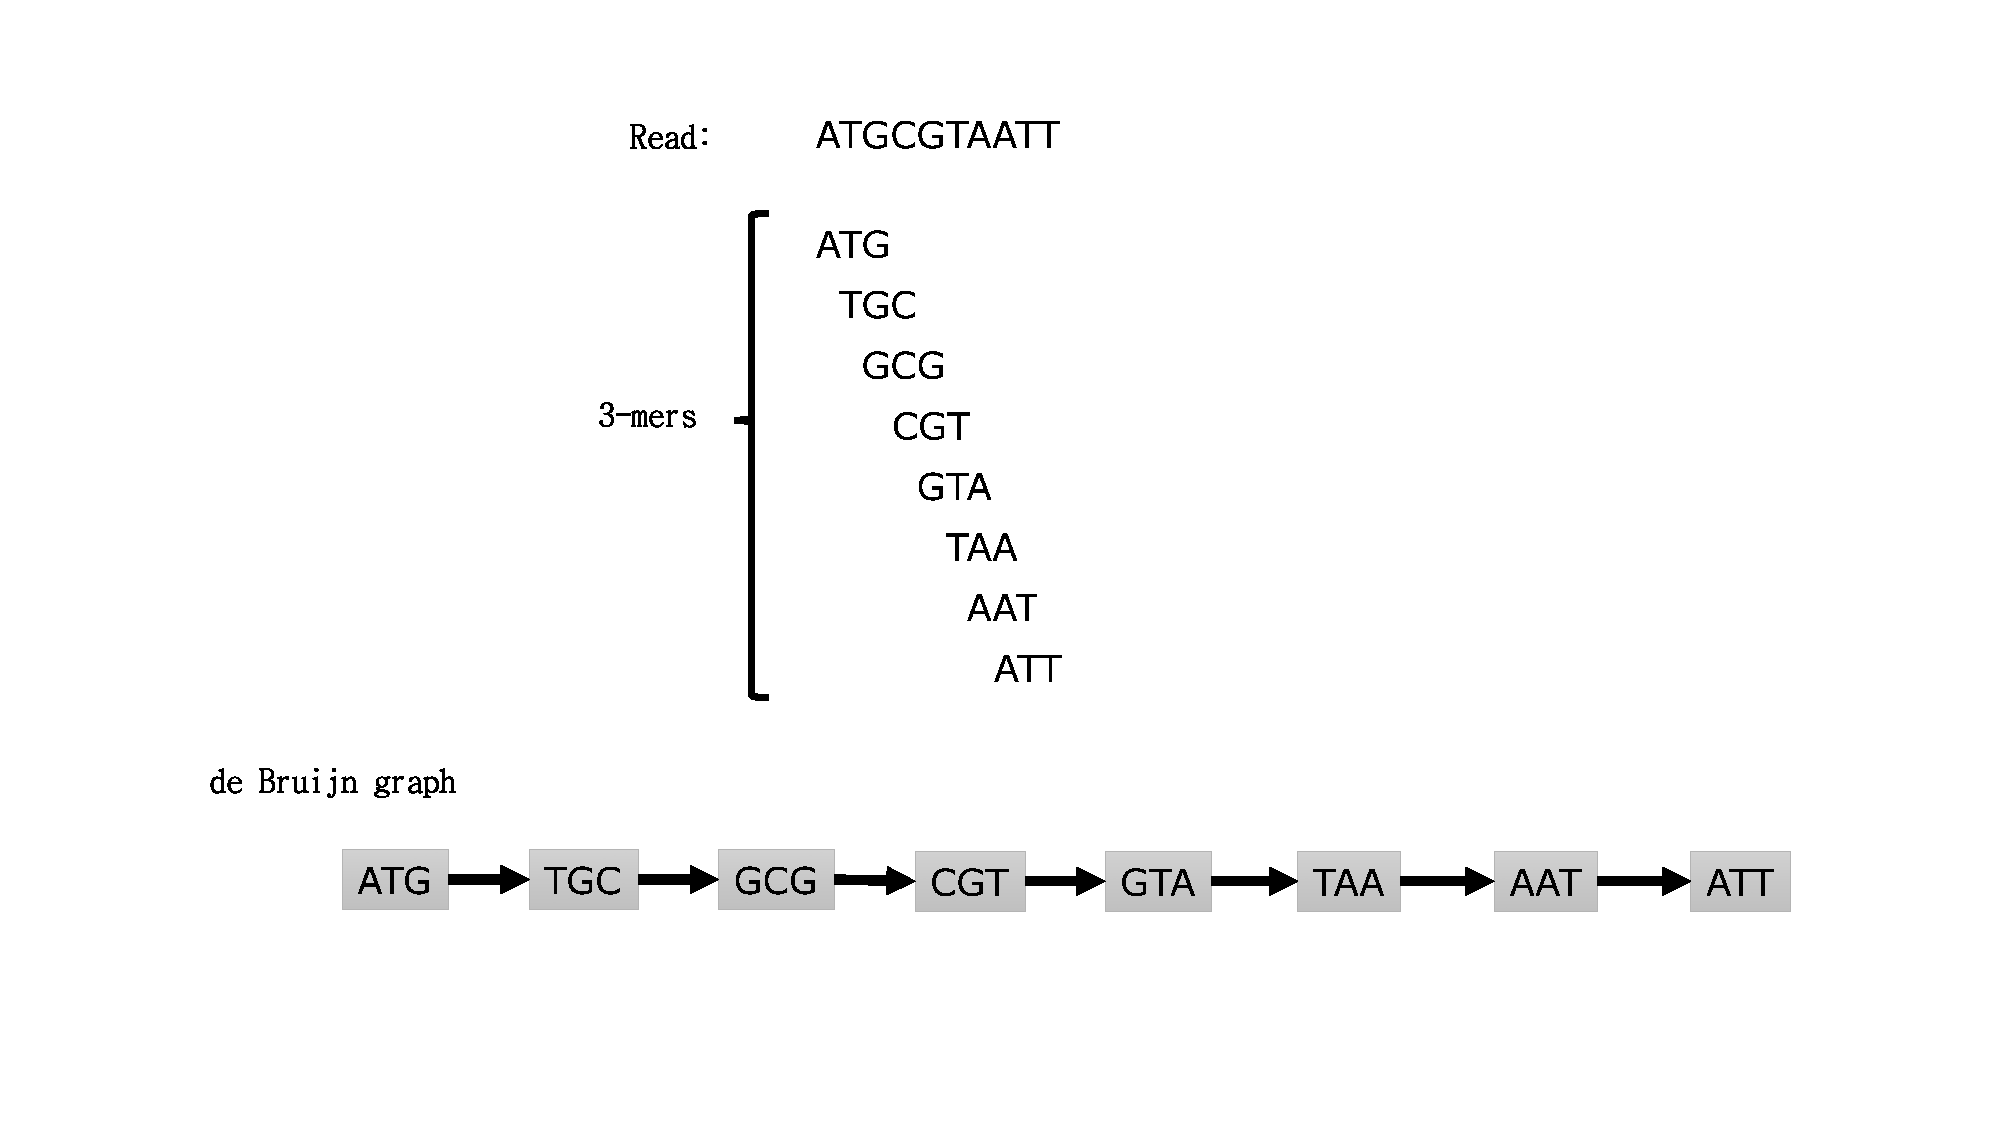
\includegraphics[scale=0.4]{Figure2_4.eps}
    \caption[De Bruijn Graph]{
         De bruijn graph for reads with $k$-mer=3.
        }
    \label{fig:Figure2.4}
  \end{figure}
\end{description}
\paragraph{}
The software package Velvet~\cite{Zerbino2008} was among the first assemblers for short reads and is now widely used. It implements an approach based on {\em de bruijn} graphs, uses information from read pairs, and implements various error correction steps after building the graph. Velvet has successfully been used to assemble bacterial genomes. The assemblers ABySS~\cite{Simpson2009} also use the {\em de bruijn} graph methods. Its advantage is that it can be run in a parallel environment and thus has the potential to assemble much larger genomes. For example, Simpson {\em et al}. demonstrate the assembly of a human genome using ABySS. SOAPdenovo~\cite{Li2008} also implements a parallel assembly algorithm based on {\em de bruijn} graphs. 
